\documentclass[aspectratio=169, table, 12pt]{beamer}
% Preamble bersama seluruh slide mata kuliah ini.
% Dipanggil dari slides/sessionXX/sessionXX.tex tepat sesudah baris
% \documentclass[aspectratio=169, table, 12pt]{beamer}
% Paket tambahan yang hanya dibutuhkan satu sesi ditulis di berkas sesi itu.

\usepackage{colortbl}
\usepackage{xcolor}
\usepackage{listings}
\usepackage{tabularx}
\usepackage{booktabs}
\usepackage{tikz}
\usepackage{pgfplots}
\pgfplotsset{compat=1.18}
\usetikzlibrary{arrows.meta, positioning, calc, fit, shapes.geometric,
	shapes.multipart, backgrounds, matrix, chains, trees}

\makeatletter
\def\input@path{{../theme/}}
\makeatother
\graphicspath{{../theme/}{../../figures/}}
\usetheme{Pradita}

\definecolor{praditagreen}{RGB}{37, 113, 71}

% Tema membuat garis tabel berwarna putih. Dikembalikan agar tabel terbaca.
\arrayrulecolor{black}
\setlength{\arrayrulewidth}{0.5pt}

\lstdefinelanguage{yaml}{
	basicstyle=\ttfamily\scriptsize,
	keywordstyle=\color{blue}\bfseries,
	commentstyle=\color{gray}\itshape,
	stringstyle=\color{red},
	showstringspaces=false,
	breaklines=true,
	frame=lines,
	numbers=none,
	backgroundcolor=\color{lightgray!10},
	tabsize=2,
	morecomment=[l]{\#}
}

\lstdefinelanguage{json}{
	basicstyle=\ttfamily\scriptsize,
	stringstyle=\color{red},
	commentstyle=\color{gray},
	breaklines=true,
	showstringspaces=false,
	tabsize=2,
	numbers=none,
	frame=lines,
	backgroundcolor=\color{lightgray!10},
	string=[s]{"}{"}
}

\lstdefinelanguage{bash}{
	keywords={},
	basicstyle=\ttfamily\scriptsize,
	ndkeywords={docker, kubectl, helm, curl, git, terraform},
	ndkeywordstyle=\color{purple}\bfseries,
	sensitive=true,
	commentstyle=\color{gray},
	numbers=none,
	breaklines=true,
	frame=lines,
	backgroundcolor=\color{lightgray!10},
	tabsize=2,
	comment=[l]{\#},
	showstringspaces=false
}

\lstdefinelanguage{http}{
	keywords={GET, POST, PUT, PATCH, DELETE, HEAD, OPTIONS, HTTP},
	basicstyle=\ttfamily\scriptsize,
	keywordstyle=\color{blue}\bfseries,
	sensitive=true,
	numbers=none,
	breaklines=true,
	frame=lines,
	backgroundcolor=\color{lightgray!10},
	tabsize=2,
	showstringspaces=false
}

\subtitle{IT40713 · Cloud-Native \& Microservices Architecture}
\author{\textbf{Alfa Yohannis}}


% Kolom X rata kiri agar spasi antarkata tidak meregang pada kolom sempit.
\newcolumntype{Y}{>{\raggedright\arraybackslash}X}

\title{\Huge Prinsip Cloud-Native\\ \vspace{10pt} dan Twelve-Factor App}

\begin{document}

\frame{\titlepage}

\begin{frame}
  \frametitle{Isi Pertemuan}
  \vspace{14pt}
  \begin{columns}[t]
    \column{0.5\textwidth}
    {\small\tableofcontents[sections={1-5}]}

    \column{0.5\textwidth}
    {\small\tableofcontents[sections={6-9}]}
  \end{columns}
\end{frame}

\begin{frame}{\hfill}
  \centering
  \Huge{\textbf{Sudah di \textit{cloud},\\mengapa masih lambat?}}
\end{frame}

\section{Tujuan dan Kerangka Bahasan}

\begin{frame}{\hfill}
  \centering
  \Huge{\textbf{Tujuan dan Kerangka Bahasan}}
\end{frame}

\begin{frame}{{\Large Tujuan Pembelajaran}}
  \vspace{10pt}
  \begin{itemize}
    \item Menjelaskan definisi \textit{cloud-native} menurut CNCF (Cloud Native
          Computing Foundation) dan perbedaannya dengan aplikasi yang sekadar
          \textit{cloud-hosted}.
    \item Menerjemahkan dua belas faktor Twelve-Factor App ke dalam dampak bisnis
          yang mudah dipahami.
    \item Menilai kesenjangan aplikasi yang ada terhadap prinsip
          \textit{cloud-native}.
  \end{itemize}
\end{frame}

\begin{frame}{{\Large Medikara+: Sudah di Cloud, Tetap Lambat}}
  \vspace{10pt}
  \begin{itemize}
    \item Berjalan di dua mesin virtual di \textit{cloud} milik vendor sejak 2023.
    \item Setiap program vaksinasi diumumkan, banyak pemesanan gagal.
    \item Satu pembaruan kecil tetap butuh dua minggu.
    \item Lokasi server berubah, cara membangun dan menjalankannya tidak.
    \item Bab ini memberi alat ukurnya: definisi CNCF dan dua belas faktor.
  \end{itemize}
\end{frame}

\section{Definisi Cloud-Native CNCF}

\begin{frame}{\hfill}
  \centering
  \Huge{\textbf{Definisi Cloud-Native CNCF}}
\end{frame}

\begin{frame}{{\Large Definisi Versi 1.1 (26 Februari 2024)}}
  \vspace{6pt}
  \begin{itemize}
    \item \textbf{Praktik:} mengembangkan, membangun, dan men-\textit{deploy}
          \textit{workload} di \textit{cloud} publik, privat, atau hibrida, secara
          terprogram dan dapat diulang.
    \item \textbf{Sifat:} keterkaitan longgar, aman, tangguh, terkelola,
          berkelanjutan, dapat diamati.
    \item \textbf{Teknologi:} \textit{container}, \textit{service mesh},
          \textit{microservices}, \textit{serverless}, dan lainnya; daftarnya tidak
          lengkap.
    \item \textbf{Hasil:} perubahan berdampak besar, sering, dapat diprediksi,
          kerja manual minimal.
  \end{itemize}
\end{frame}

\begin{frame}{{\Large Membaca Definisi dari Kiri ke Kanan}}
  \centering
  \eadiagram{../../figures/ch05-definisi-cncf.tex}
\end{frame}

\begin{frame}{{\Large Dari Versi 1.0 (2018) ke Versi 1.1 (2024)}}
  \vspace{4pt}
  \footnotesize
  \begin{tabularx}{\textwidth}{|p{2.6cm}|Y|Y|}
    \hline
    \textbf{Aspek} & \textbf{Versi 1.0} & \textbf{Versi 1.1} \\
    \hline
    Pokok kalimat & Teknologi & Praktik \\
    \hline
    Yang dibangun & Aplikasi yang dapat diskalakan & \textit{Workload}, terprogram
      dan dapat diulang \\
    \hline
    Sifat sistem & Longgar, tangguh, terkelola, dapat diamati & Ditambah aman dan
      berkelanjutan \\
    \hline
    Contoh teknologi & Lima contoh & Ditambah \textit{multi-tenancy} dan
      \textit{serverless} \\
    \hline
  \end{tabularx}

  \vspace{8pt}
  \small Membeli alat tidak otomatis membuat organisasi \textit{cloud-native}.
\end{frame}

\begin{frame}{{\Large Cloud-Hosted dan Cloud-Native}}
  \vspace{10pt}
  \begin{itemize}
    \item Ukurannya sifat sistem, bukan lokasi server.
    \item Medikara+: dua mesin virtual, naik kapasitas 40 menit dengan semua
          pengguna terputus, pembaruan dua minggu. \textit{Cloud-hosted}.
    \item Misalkan bank daerah di pusat data sendiri, tetapi rilis otomatis
          dalam 30 menit: lebih dekat ke \textit{cloud-native}.
    \item Keduanya ujung sebuah rentang; sebagian besar aplikasi ada di tengah.
  \end{itemize}
\end{frame}

\section{Twelve-Factor App}

\begin{frame}{\hfill}
  \centering
  \Huge{\textbf{Twelve-Factor App}}
\end{frame}

\begin{frame}{{\Large Asal-Usul dan Status Sekarang}}
  \vspace{10pt}
  \begin{itemize}
    \item Ditulis Adam Wiggins, salah satu pendiri Heroku, pada 2011.
    \item Teks yang dibaca sekarang terakhir diperbarui pada 2017.
    \item Sejak 12 November 2024 menjadi proyek \textit{open source} yang dikelola
          komunitas.
    \item Hoffman (2016) menambah tiga: \textit{API first}, telemetri, serta
          autentikasi dan otorisasi.
    \item Kartu skor mencatat tanggal akses dan versi teks faktor.
  \end{itemize}
\end{frame}

\begin{frame}{{\Large Dua Belas Faktor dalam Tiga Kelompok}}
  \centering
  \eadiagram{../../figures/ch05-tiga-kelompok.tex}
\end{frame}

\begin{frame}{{\Large Alat Penilaian, Bukan Dogma}}
  \vspace{10pt}
  \begin{itemize}
    \item Seperti pemeriksaan kesehatan berkala: tidak semua angka harus
          sempurna.
    \item Yang dibaca: angka yang menyimpang dan seberapa berbahaya.
    \item Medikara+ (310.000 pengguna, beban naik turun): hampir semua faktor
          relevan.
    \item Rekap lembur bulanan (12 pengguna): faktor skala hampir tidak relevan,
          konfigurasi dan \textit{log} tetap penting.
  \end{itemize}
\end{frame}

\section{Kode, Konfigurasi, dan Backing Service}

\begin{frame}{\hfill}
  \centering
  \Huge{\textbf{Kode, Konfigurasi,\\dan Backing Service}}
\end{frame}

\begin{frame}{{\Large Kelompok A: Faktor I sampai IV}}
  \vspace{10pt}
  \begin{itemize}
    \item \textbf{I \textit{Codebase}:} satu basis kode, dipasang di banyak tempat.
    \item \textbf{II \textit{Dependencies}:} pustaka dan versinya ditulis eksplisit.
    \item \textbf{III \textit{Config}:} yang berbeda antarlokasi disimpan di
          lingkungan, bukan di kode.
    \item \textbf{IV \textit{Backing services}:} basis data, BPJS Kesehatan, dan
          SATUSEHAT dipasang lewat konfigurasi.
    \item Uji sederhana: bila kode dibuka ke publik, adakah kredensial yang bocor?
  \end{itemize}
\end{frame}

\begin{frame}{{\Large Satu Kode, Lima Release}}
  \centering
  \eadiagram{../../figures/ch05-satu-kode-banyak-deploy.tex}
\end{frame}

\begin{frame}{{\Large Kasus Medikara: Konfigurasi SIMRS di Lima Rumah Sakit}}
  \vspace{10pt}
  \begin{itemize}
    \item Versi 3.9 di Bandung sampai 5.2 di Jakarta, salinan kode masing-masing.
    \item 37 nilai konfigurasi tertanam di kode; 9 berupa kata sandi atau kunci
          akses.
    \item Misalkan alamat integrasi BPJS Kesehatan berubah: 2 hari kerja per rumah
          sakit, total 10 hari kerja.
    \item Konfigurasi di lingkungan: satu hari kerja untuk kelima rumah sakit.
  \end{itemize}
\end{frame}

\section{Build, Proses, dan Skala}

\begin{frame}{\hfill}
  \centering
  \Huge{\textbf{Build, Proses, dan Skala}}
\end{frame}

\begin{frame}{{\Large Kelompok B: Faktor V sampai IX}}
  \vspace{10pt}
  \begin{itemize}
    \item \textbf{V:} \textit{build}, \textit{release}, \textit{run} terpisah;
          \textit{release} bernomor dan tidak diubah.
    \item \textbf{VI:} proses tanpa \textit{state}; sesi di penyimpanan bersama.
    \item \textbf{VII:} aplikasi melayani sendiri lewat \textit{port}.
    \item \textbf{VIII:} kapasitas ditambah dengan menambah proses.
    \item \textbf{IX:} cepat menyala, berhenti rapi saat \texttt{SIGTERM}.
  \end{itemize}
\end{frame}

\begin{frame}{{\Large Penskalaan Vertikal dan Horizontal}}
  \vspace{4pt}
  \footnotesize
  \begin{tabularx}{\textwidth}{|p{2.8cm}|Y|Y|}
    \hline
    \textbf{Aspek} & \textbf{Vertikal (\textit{scale up})} &
      \textbf{Horizontal (\textit{scale out})} \\
    \hline
    Cara & Server lebih besar & Server atau proses yang sama ditambah \\
    \hline
    Waktu menambah & Puluhan menit, nyala ulang & Menit atau detik \\
    \hline
    Satu server mati & Seluruh layanan berhenti & Server lain tetap melayani \\
    \hline
    Syarat aplikasi & Hampir tidak ada & Tanpa \textit{state}, cepat menyala \\
    \hline
    Pola biaya & Server besar dibayar terus & Turun lagi setelah jam sibuk \\
    \hline
  \end{tabularx}
\end{frame}

\begin{frame}{{\Large Sesi di Memori Server Menghambat Penskalaan}}
  \centering
  \eadiagram{../../figures/ch05-sesi-skala.tex}
\end{frame}

\begin{frame}{{\Large Diagram Konsep Bab 5}}
  \centering
  {\small\bfseries Aplikasi stateless memisahkan proses dari data persisten}\par\medskip
  \adjustbox{width=0.96\textwidth,height=0.7\textheight,keepaspectratio}{%
    % Diagram konsep Bab 5: Aplikasi stateless memisahkan proses dari data persisten.
% Dibangkitkan tools/render-diagrams.py dari figures/chapter-diagrams.json;
% ubah data JSON lalu jalankan ulang skrip, jangan sunting berkas ini langsung.
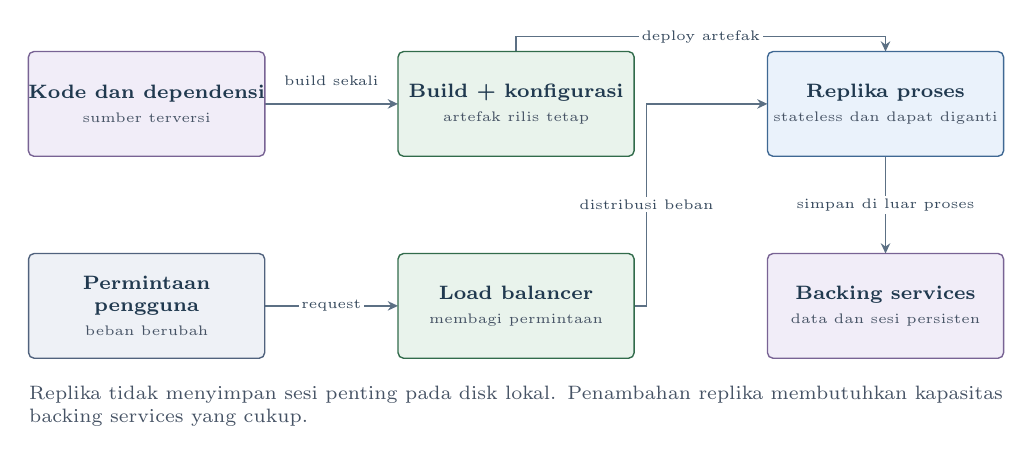
\begin{tikzpicture}[
  x=0.92cm, y=0.95cm,
  kotak konsep/.style={draw, line width=0.5pt, rounded corners=2pt,
    align=center, minimum width=2.999cm,
    minimum height=1.330cm, inner sep=0pt, font=\scriptsize,
    text=konsepJudul},
  peran actor/.style={kotak konsep, fill=konsepIsiActor, draw=konsepGarisActor},
  peran service/.style={kotak konsep, fill=konsepIsiService, draw=konsepGarisService},
  peran control/.style={kotak konsep, fill=konsepIsiControl, draw=konsepGarisControl},
  peran data/.style={kotak konsep, fill=konsepIsiData, draw=konsepGarisData},
  peran outcome/.style={kotak konsep, fill=konsepIsiOutcome, draw=konsepGarisOutcome},
  peran risk/.style={kotak konsep, fill=konsepIsiRisk, draw=konsepGarisRisk},
  panah konsep/.style={-{Stealth[length=1.3mm, width=1.2mm]}, line width=0.6pt,
    draw=konsepPanah},
  panah putus/.style={panah konsep, draw=konsepPanahPutus,
    dash pattern=on 2.5pt off 1.5pt},
  label panah/.style={font=\tiny, align=center, fill=white,
    inner sep=1pt, text=konsepLabel},
  catatan/.style={font=\scriptsize, align=left, anchor=north west,
    inner sep=0pt, text width=12.383cm, text=konsepTeks,
    execute at begin node={\hyphenpenalty=10000\hbadness=10000\relax}},
]
  \definecolor{konsepIsiActor}{HTML}{EEF1F6}
  \definecolor{konsepGarisActor}{HTML}{50627D}
  \definecolor{konsepIsiService}{HTML}{EAF2FB}
  \definecolor{konsepGarisService}{HTML}{3F6893}
  \definecolor{konsepIsiControl}{HTML}{E9F3EC}
  \definecolor{konsepGarisControl}{HTML}{316B4B}
  \definecolor{konsepIsiData}{HTML}{F1EDF8}
  \definecolor{konsepGarisData}{HTML}{786394}
  \definecolor{konsepIsiOutcome}{HTML}{E4F2EC}
  \definecolor{konsepGarisOutcome}{HTML}{236C57}
  \definecolor{konsepIsiRisk}{HTML}{FCEDE7}
  \definecolor{konsepGarisRisk}{HTML}{B36947}
  \definecolor{konsepJudul}{HTML}{20394F}
  \definecolor{konsepTeks}{HTML}{455264}
  \definecolor{konsepLabel}{HTML}{35485C}
  \definecolor{konsepPanah}{HTML}{5C7084}
  \definecolor{konsepPanahPutus}{HTML}{A15D40}
  % Panah dan label lebih dahulu; kotak menutupi sisa latar label.
  \draw[panah konsep] (0.93,0) -- (2.77,0);
  \draw[panah konsep] (4.4,0.7) -- (4.4,0.9) -- (9.5,0.9) -- (9.5,0.7);
  \draw[panah konsep] (0.93,-2.7) -- (2.77,-2.7);
  \draw[panah konsep] (6.03,-2.7) -- (6.2,-2.7) -- (6.2,0) -- (7.87,0);
  \draw[panah konsep] (9.5,-0.7) -- (9.5,-2);
  \node[label panah] at (1.85,0.31) {build sekali};
  \node[label panah] at (6.95,0.9) {deploy artefak};
  \node[label panah] at (1.85,-2.7) {request};
  \node[label panah] at (6.2,-1.35) {distribusi beban};
  \node[label panah] at (9.5,-1.35) {simpan di luar proses};
  \node[peran data] (kode) at (-0.7,0)
    {\textbf{Kode dan dependensi}\\[0.5pt]{\tiny\color{konsepTeks}sumber terversi}};
  \node[peran control] (rilis) at (4.4,0)
    {\textbf{Build + konfigurasi}\\[0.5pt]{\tiny\color{konsepTeks}artefak rilis tetap}};
  \node[peran service] (replika) at (9.5,0)
    {\textbf{Replika proses}\\[0.5pt]{\tiny\color{konsepTeks}stateless dan dapat diganti}};
  \node[peran actor] (klien) at (-0.7,-2.7)
    {\textbf{Permintaan}\\\textbf{pengguna}\\[0.5pt]{\tiny\color{konsepTeks}beban berubah}};
  \node[peran control] (lb) at (4.4,-2.7)
    {\textbf{Load balancer}\\[0.5pt]{\tiny\color{konsepTeks}membagi permintaan}};
  \node[peran data] (data) at (9.5,-2.7)
    {\textbf{Backing services}\\[0.5pt]{\tiny\color{konsepTeks}data dan sesi persisten}};
  \node[catatan] at (-2.33,-3.77)
    {Replika tidak menyimpan sesi penting pada disk lokal. Penambahan replika membutuhkan kapasitas backing services yang cukup.};
\end{tikzpicture}
}
\end{frame}

\begin{frame}{{\Large Kasus Medikara: Lonjakan saat Program Vaksinasi}}
  \vspace{10pt}
  \begin{itemize}
    \item Misalkan dalam 20 menit pengguna aktif naik dari 1.200 menjadi 9.600.
    \item Waktu respons 1,5 detik menjadi 14 detik; 23 persen pemesanan gagal.
    \item Vendor naik vertikal 8 ke 16 inti prosesor: 40 menit, semua sesi hilang.
    \item Mesin baru butuh 11 menit untuk menyala.
    \item Kesenjangan: faktor VI, VIII, dan IX.
  \end{itemize}
\end{frame}

\section{Lingkungan, Log, dan Tugas Admin}

\begin{frame}{\hfill}
  \centering
  \Huge{\textbf{Lingkungan, Log,\\dan Tugas Admin}}
\end{frame}

\begin{frame}{{\Large Kelompok C: Faktor X sampai XII}}
  \vspace{10pt}
  \begin{itemize}
    \item \textbf{X \textit{Dev/prod parity}:} persempit kesenjangan waktu, orang,
          dan alat.
    \item \textbf{XI \textit{Logs}:} aplikasi menulis ke \texttt{stdout}, platform
          yang mengumpulkan.
    \item \textbf{XII \textit{Admin processes}:} tugas sekali jalan memakai
          \textit{release} dan konfigurasi yang sama.
    \item Analogi: kamera pengawas mengirim rekaman ke ruang kendali, tidak
          menyimpannya sendiri.
  \end{itemize}
\end{frame}

\begin{frame}{{\Large Kasus Medikara: Pertanyaan Audit Laboratorium}}
  \vspace{10pt}
  \begin{itemize}
    \item Auditor meminta daftar petugas yang membuka hasil lab dalam 90 hari.
    \item \textit{Log} hanya tujuh hari, berkas lokal di tiga server.
    \item Mengumpulkan tujuh hari itu saja butuh tiga hari kerja.
    \item Misalkan gangguan enam jam pada Maret 2026: versi basis data uji berbeda
          dari produksi.
    \item Kesenjangan: faktor XI dan X.
  \end{itemize}
\end{frame}

\section{Immutable dan Deklaratif}

\begin{frame}{\hfill}
  \centering
  \Huge{\textbf{Immutable dan Deklaratif}}
\end{frame}

\begin{frame}{{\Large Server yang Dirawat dan Server yang Diganti}}
  \centering
  \eadiagram{../../figures/ch05-immutable.tex}

  \vspace{4pt}
  \footnotesize Server SIMRS Depok (2019): pengganti butuh 4 hari. Misalkan dari
  definisi tertulis: sekitar 45 menit.
\end{frame}

\begin{frame}{{\Large Langkah Manual dan Konfigurasi Deklaratif}}
  \vspace{10pt}
  \begin{itemize}
    \item Imperatif menulis langkah; deklaratif menulis keadaan akhir.
    \item Analogi: petunjuk belok kiri dan kanan dibandingkan alamat tujuan di
          aplikasi peta.
    \item Deklaratif: hasil sama setiap kali, penyimpangan dideteksi.
    \item Biayanya: alat, keterampilan, dan disiplin tanpa ubah langsung di
          server.
    \item Jembatan ke \textit{container} (Bab 8) dan GitOps (Bab 13).
  \end{itemize}
\end{frame}

\section{Aktivitas}

\begin{frame}{\hfill}
  \centering
  \Huge{\textbf{Aktivitas: Kartu Skor\\Kesenjangan Cloud-Native}}
\end{frame}

\begin{frame}{{\Large Aktivitas: Tujuan dan Peran}}
  \vspace{10pt}
  \begin{itemize}
    \item Menilai 2 sampai 3 aplikasi inti terhadap dua belas faktor.
    \item Anggota teknis: menjelaskan faktor dan mengumpulkan bukti.
    \item Anggota non-teknis: menulis dampak bisnis dengan angka.
    \item Luaran: kartu skor dan ringkasan satu halaman untuk C2.
    \item Berkas: \berkas{sources/chapter05/kartu-skor-twelve-factor.xlsx}.
  \end{itemize}
\end{frame}

\begin{frame}{{\Large Aktivitas: Langkah dan Skala Skor}}
  \vspace{6pt}
  \begin{columns}[t]
    \column{0.55\textwidth}
    \small
    \begin{enumerate}
      \item Pilih aplikasi dari portofolio Bab 4.
      \item Pelajari arti setiap faktor.
      \item Kumpulkan bukti tanpa data rahasia.
      \item Beri skor dengan satu kalimat bukti.
      \item Tulis dampak bisnis skor 0 dan 1.
      \item Tandai tiga kesenjangan terpenting.
    \end{enumerate}
    \column{0.42\textwidth}
    \small
    \begin{tabularx}{\linewidth}{|p{0.8cm}|Y|}
      \hline
      \textbf{Skor} & \textbf{Arti} \\
      \hline
      0 & Belum dipenuhi \\
      \hline
      1 & Sebagian kecil \\
      \hline
      2 & Sebagian besar \\
      \hline
      3 & Dipenuhi \\
      \hline
      TR & Tidak relevan \\
      \hline
    \end{tabularx}
  \end{columns}
\end{frame}

\begin{frame}{{\Large Contoh Kartu Skor Medikara Health}}
  \vspace{2pt}
  \scriptsize
  \begin{columns}[t]
    \column{0.48\textwidth}
    \begin{tabularx}{\linewidth}{|Y|c|c|c|}
      \hline
      \textbf{Faktor} & \textbf{SIMRS} & \textbf{M+} & \textbf{Lab} \\
      \hline
      I \textit{Codebase} & 0 & 2 & 2 \\
      \hline
      II \textit{Dependencies} & 1 & 2 & 1 \\
      \hline
      III \textit{Config} & 0 & 1 & 1 \\
      \hline
      IV \textit{Backing services} & 1 & 2 & 1 \\
      \hline
      V \textit{Build, release, run} & 0 & 1 & 1 \\
      \hline
      VI \textit{Processes} & 1 & 0 & 2 \\
      \hline
    \end{tabularx}
    \column{0.48\textwidth}
    \begin{tabularx}{\linewidth}{|Y|c|c|c|}
      \hline
      \textbf{Faktor} & \textbf{SIMRS} & \textbf{M+} & \textbf{Lab} \\
      \hline
      VII \textit{Port binding} & 1 & 2 & 1 \\
      \hline
      VIII \textit{Concurrency} & 0 & 1 & 1 \\
      \hline
      IX \textit{Disposability} & 0 & 1 & 1 \\
      \hline
      X \textit{Dev/prod parity} & 0 & 1 & 1 \\
      \hline
      XI \textit{Logs} & 1 & 1 & 0 \\
      \hline
      XII \textit{Admin processes} & 1 & 2 & 1 \\
      \hline
    \end{tabularx}
  \end{columns}

  \vspace{8pt}
  \small Jumlah dari 36: SIMRS Bogor 6, Medikara+ (M+) 16, sistem lab 13.
  Terpenting: VI pada Medikara+, III pada SIMRS, XI pada lab.
\end{frame}

\section{Ringkasan dan Latihan}

\begin{frame}{{\Large Ringkasan}}
  \vspace{10pt}
  \begin{itemize}
    \item CNCF 1.1 menilai praktik dan sifat sistem, bukan lokasi atau merek alat.
    \item Dua belas faktor, tiga pertanyaan: dipasang di banyak lokasi, kapasitas
          dalam menit, dirawat dan diaudit dengan cepat.
    \item Setiap kesenjangan punya dampak bisnis yang dapat dihitung.
    \item \textit{Immutable infrastructure} dan konfigurasi deklaratif menjaga
          server tetap sama dengan definisinya.
    \item \textit{Cloud-native} adalah sifat yang dibuktikan, bukan lokasi yang
          ditempati.
  \end{itemize}
\end{frame}

\begin{frame}{{\Large Latihan}}
  \vspace{10pt}
  \begin{enumerate}
    \item Medikara+ sering lambat setiap kali program vaksinasi diumumkan. Faktor
          mana yang paling relevan, dan mengapa?
    \item Jelaskan dengan bahasa non-teknis mengapa aplikasi yang menyimpan sesi
          di memori server sulit diskalakan.
    \item Apakah semua aplikasi organisasi perlu memenuhi dua belas faktor?
          Berikan satu contoh yang tidak perlu beserta alasannya.
  \end{enumerate}
\end{frame}

\end{document}
